\documentclass{article}
\usepackage[utf8]{inputenc}
\usepackage[portuguese]{babel}
\usepackage{csquotes}
\usepackage{graphicx}
\usepackage{adjustbox}
\usepackage{lipsum}
\usepackage[backend=biber,autolang=other,
  bibencoding=utf8,style=authoryear-ibid,
  ibidtracker=true]{biblatex}

\addbibresource{4obras.bib}

\title{Análise Sumária de 4 obras da História da Arte} \date{10 de
  Dezembro de 2015} \author{João Távora \\Faculdade de Belas Artes da
  Universidade de Lisboa}

\begin{document}

\maketitle

\section{Cabeça do Rei Senuseret III}

\begin{figure}
\centering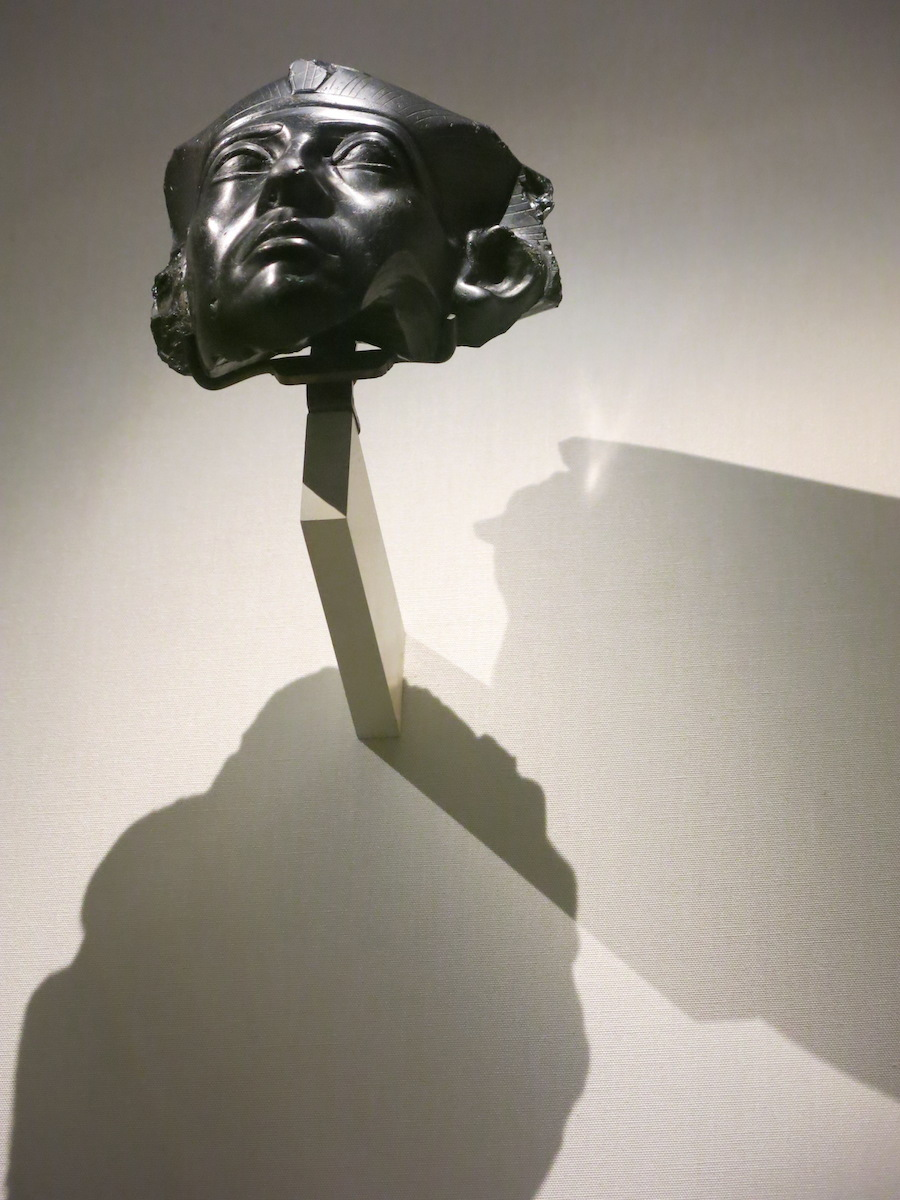
\includegraphics[height=0.3\textheight,keepaspectratio]
                          {senuseret.jpg}
  \caption{Cabeça do Rei Senuseret III em pedra obsidiana}.
  \label{fig:1}
\end{figure}

A cabeça da figura \ref{fig:1}, visitada no Museu Gulbenkian, faria
parte de uma estatueta de corpo inteiro. É feita de obsidiana, vidro
vulcânico de grande dureza e fragilidade, e por isso muito dificil de
trabalhar. Os materiais duros eram preferidos pelos Egípcios e eram
indicados para as representações físicas faraónicas, que se pretendiam
que conservassem a alma no caso do corpo mortal se deteriorar. O Faraó
tem na sua cabeça, um toucado glissado encimado pelo ``eucos'',
símbolo do poder real.

Existem várias estátuas deste Rei no museu Britânico em Londres
(\cite{wiki-senuseret}), mas são em granito e estão razoavelmente
danificadas.

No museu de Brooklin em Nova Iorque, sabemos de uma outra estátua em
granito, mais completa. Nesta, o Faraó enverga o toucado, ou
\emph{nemes}, com uma cobra na frente, o \emph{shendyt}, um
saiote. Entre as suas pernas é visível uma cauda de boi. Debaixo dos
seus pés estão nove arcos, que simbolizam os inimigos tradicionais de
Egipto submetidos ao seu poder. Ao contrário dos seus antecessores,
que eram representados com traços faciais idealizados, o Faraó
Senuseret apresenta pálpebras pesadas, bochecas bem desenhadas, e
lábios franzidos. Segundo \cite{wiki-senuseret}, não se conhecem as
razões desta mudança, mas as imitações destas características por reis
posteriores sugerem que esta representação se destinava a transmitir
as qualidades virtuosas do soberano.

Senuseret III é um Faraó razoavelmente importante na história do
Egipto, e é considerado o mais influente da XII dinastia, do qual ele
é o quinto monarca. Segundo \cite{wiki-senuseret}, conta-se parte da
construção do Canal dos Faraós entre os feitos realizados durante o
seu reinado. Este canal é precursor do Canal do Suez, ligando
navegavelmente o Mar Vermelho ao Nilo, e portanto ao
Mediterrâneo. Além desta suposição, parece confirmado que Senuseret
III construiu mesmo um canal através da primeira catarata do Nilo
(\cite{wiki-breasted})

O Faraó é recordado pela sua iniciativa militar de expansão até aos
reunos da Núbia, contando-se várias campanhas desde o ano 8 do seu
reinado, em 1870, até ao ano 19. Durante estas campanhas erigiu
grandes fortes em Buhem, Semna, Toshka e Uronarti. A sua presença em
Semna foi tão forte que este Faraó lá era venerado como divindade.

A pirâmide que o homenageia foi construida em Dahshur, a norte da
pirâmide vermelhade Snefery. Entre as pirâmides da XII dinastia, a de
Senuseret é mais vasta e de concepção religiosa mais complexa. Segundo
\cite{wiki-wegner}, subsistem dúvidas acerca de se Senuseret terá
realmente sido enterrado em Dashur, ou no complexo funerário mais
sofisticado de Abydos. Dadas as riquezas que normalmente era colocadas
nas tumbas dos Faraós para os acompanhar na vida eterna, é comum e
encontrar estratégias para ludibriar potenciais ladrões.

Outra curiosidade acerca de Senuseret III, é que de acordo com com
Wegner existe um papiro no museu de Berlim que demonstra que terá
havido um período de co-regência com o seu filho Amenemhat III.

\section{Torso da Deusa Vénus Anadiómena}

\begin{figure}
\centering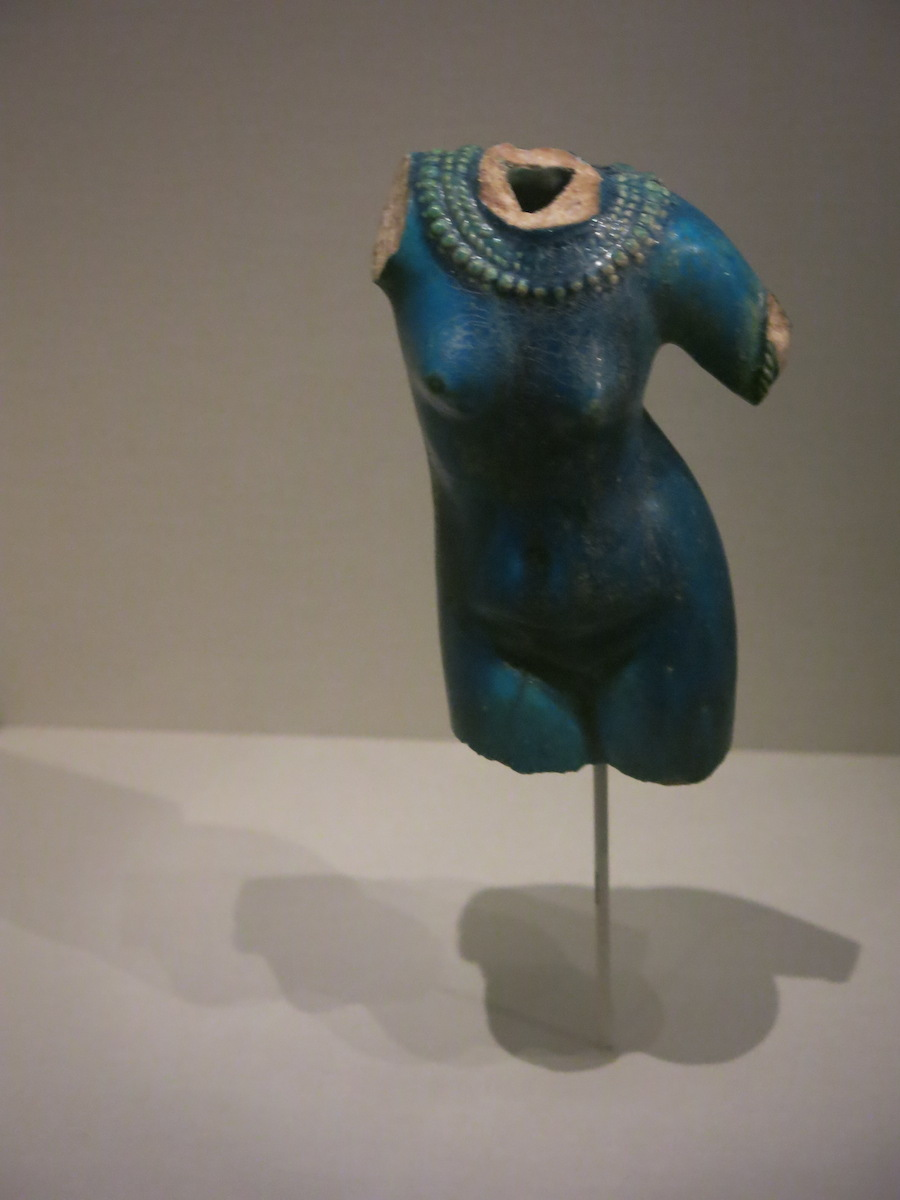
\includegraphics[height=0.3\textheight,keepaspectratio]
                          {venus.jpg}
  \caption{Torso da Deusa Vénus Anadiómena}.
  \label{fig:2}
\end{figure}

Esta peça (figura \ref{fig:2}), visitável no Museu Gulbenkian, é uma
estatueta em terracota azul envernizada. Reflecte a influência
clássica própria da época greco-romana entre 30 AC e 300DC.

A deusa, saindo das águas, tem o corpo levemente inclinado para a sua
esquerda, naquilo que se adivinha ser a pose clássica do contraposto,
num movimento ondulante e expressivo que é estranho aos cânones
egípcios. Junto do pescoço, ornamentada com um colar de três voltas,
existe um corte que mostra ser oco o interior da peça, pelo que poderá
tratar-se não apenas de uma estatueta mas de um recipiente
antropomorfo.

A época greco-romana no Egipto, também conhecida como período
helenístico, alexandrino, ou Egipto Ptolomaico, dura cerca de 300 anos
desde que Ptolomeu I Soter se tornou rei do Egipto em 305 A.C. até que
a rainha Cleópatra VII foi derrotada e o Egipto passou a ser integrado
no Império Romano como província. Culturalmente, este período
caracteriza-se por um auge, fundamentalmente em Alexandria. Esta
cidade acolheu uma grande quantidade de escritores excelentes e
converteu-se no centro literário e cultural da região. Sob a protecção
e patrocínio de Ptolomeu II, sabemos grande poetas como Calímaco,
Teócrito e Apolónio de Rodes lá residiram e formaram uma escola
literária e artística.

O nome \emph{anadiómena} significa realmente ``saída do mar'' e é
baseada numa respresentação iconográfica tornada famosa pelo pintor
grego Apeles. A representação original desapareceu, bem como todos os
quadros deste artística, mas encontra-se descrita na \emph{Naturalis
  Historiæ} de Plínio, onde se menciona, como curiosidade, que o
pintor terá usado Campaspe, concubina de Alexandre Mago, como o seu
modelo (\cite{wiki-anadiomena}). Ainda segundo Ateneo de Náucratis, a
ideia da deusa sainda do mar inspirou-se na cortesã Friné, apelido de
Mnesarete, que durante os festivais Eleusinos e dedicados ao deus
Poséidon nadava nua livremente pelo mar.

Friné era amante de Praxíteles (ca. 400 A.C, Atenas), escultor que
terá criado várias esculturas de Afrodite tendo a cortesã como
modelo. Seundo \cite{wiki-frine}, Praxíteles ofereu a Friné, como
pagamento pelos seus serviços, uma qualquer estátua do seu atelier à
sua escolha. Friné, sabendo pouco de arte, não soube decidir-se pela
melhor peça e, desta forma, resolveu urdir um plano: deu instruções a
uma servente sua que em certa ocasião, irrompesse pela sala onde
estava Praxíteles dizendo que o seu atelier estava em
cahams. Praxíteles terá exclamado: ``Salvem as minha Eros!''. Assim
Friné soube que essa era a obra predilecta do escultor e foi a que
acabou por escolher, oferendo-a de seguida à sua cidade natal de Tespias.

Acerca de Friné conta-se ainda o episódio do seu julgamento por
impiedade, delito muito grave na Grécia antiga (recorde-se que foi o
mesmo delito que levou Sócrates à sua condenação à morte), devido à
constante comparação entre a sua beleza e a da deusa Afrodite. Segundo
contam os relatos, por petição de Praxíteles, foi defendida no
julgamento pelo orador Hipérides. Hipérides foi incapaz de convencer
os juízes com o seu discurso, e desta forma, como último recurso,
recorreu ao amor e à beleza, fazendo desnudar-se Friné ante o
tribunal, argumentando que não seria justo privar o mundo de tal
beleza, que era um monumento vivo à deusa. Com esta estratégia, terá
conseguido convencer os juízes, que a absolveram unanimemente.

Esta cena dramática é representada muito mais tarde numa pintura do
pintor academista francês Jean-Léon Gérôme, que prezava ainda temas
históricos e mitológicos no século XIX. Nessa pintura de grandes
dimensões (figura \ref{fig:3}) é curioso verificar como a pose em que
se encontra a figura da concubina é precisamente a mesma da estatueta
do museu Gulbenkian em Lisboa.

\begin{figure}
\centering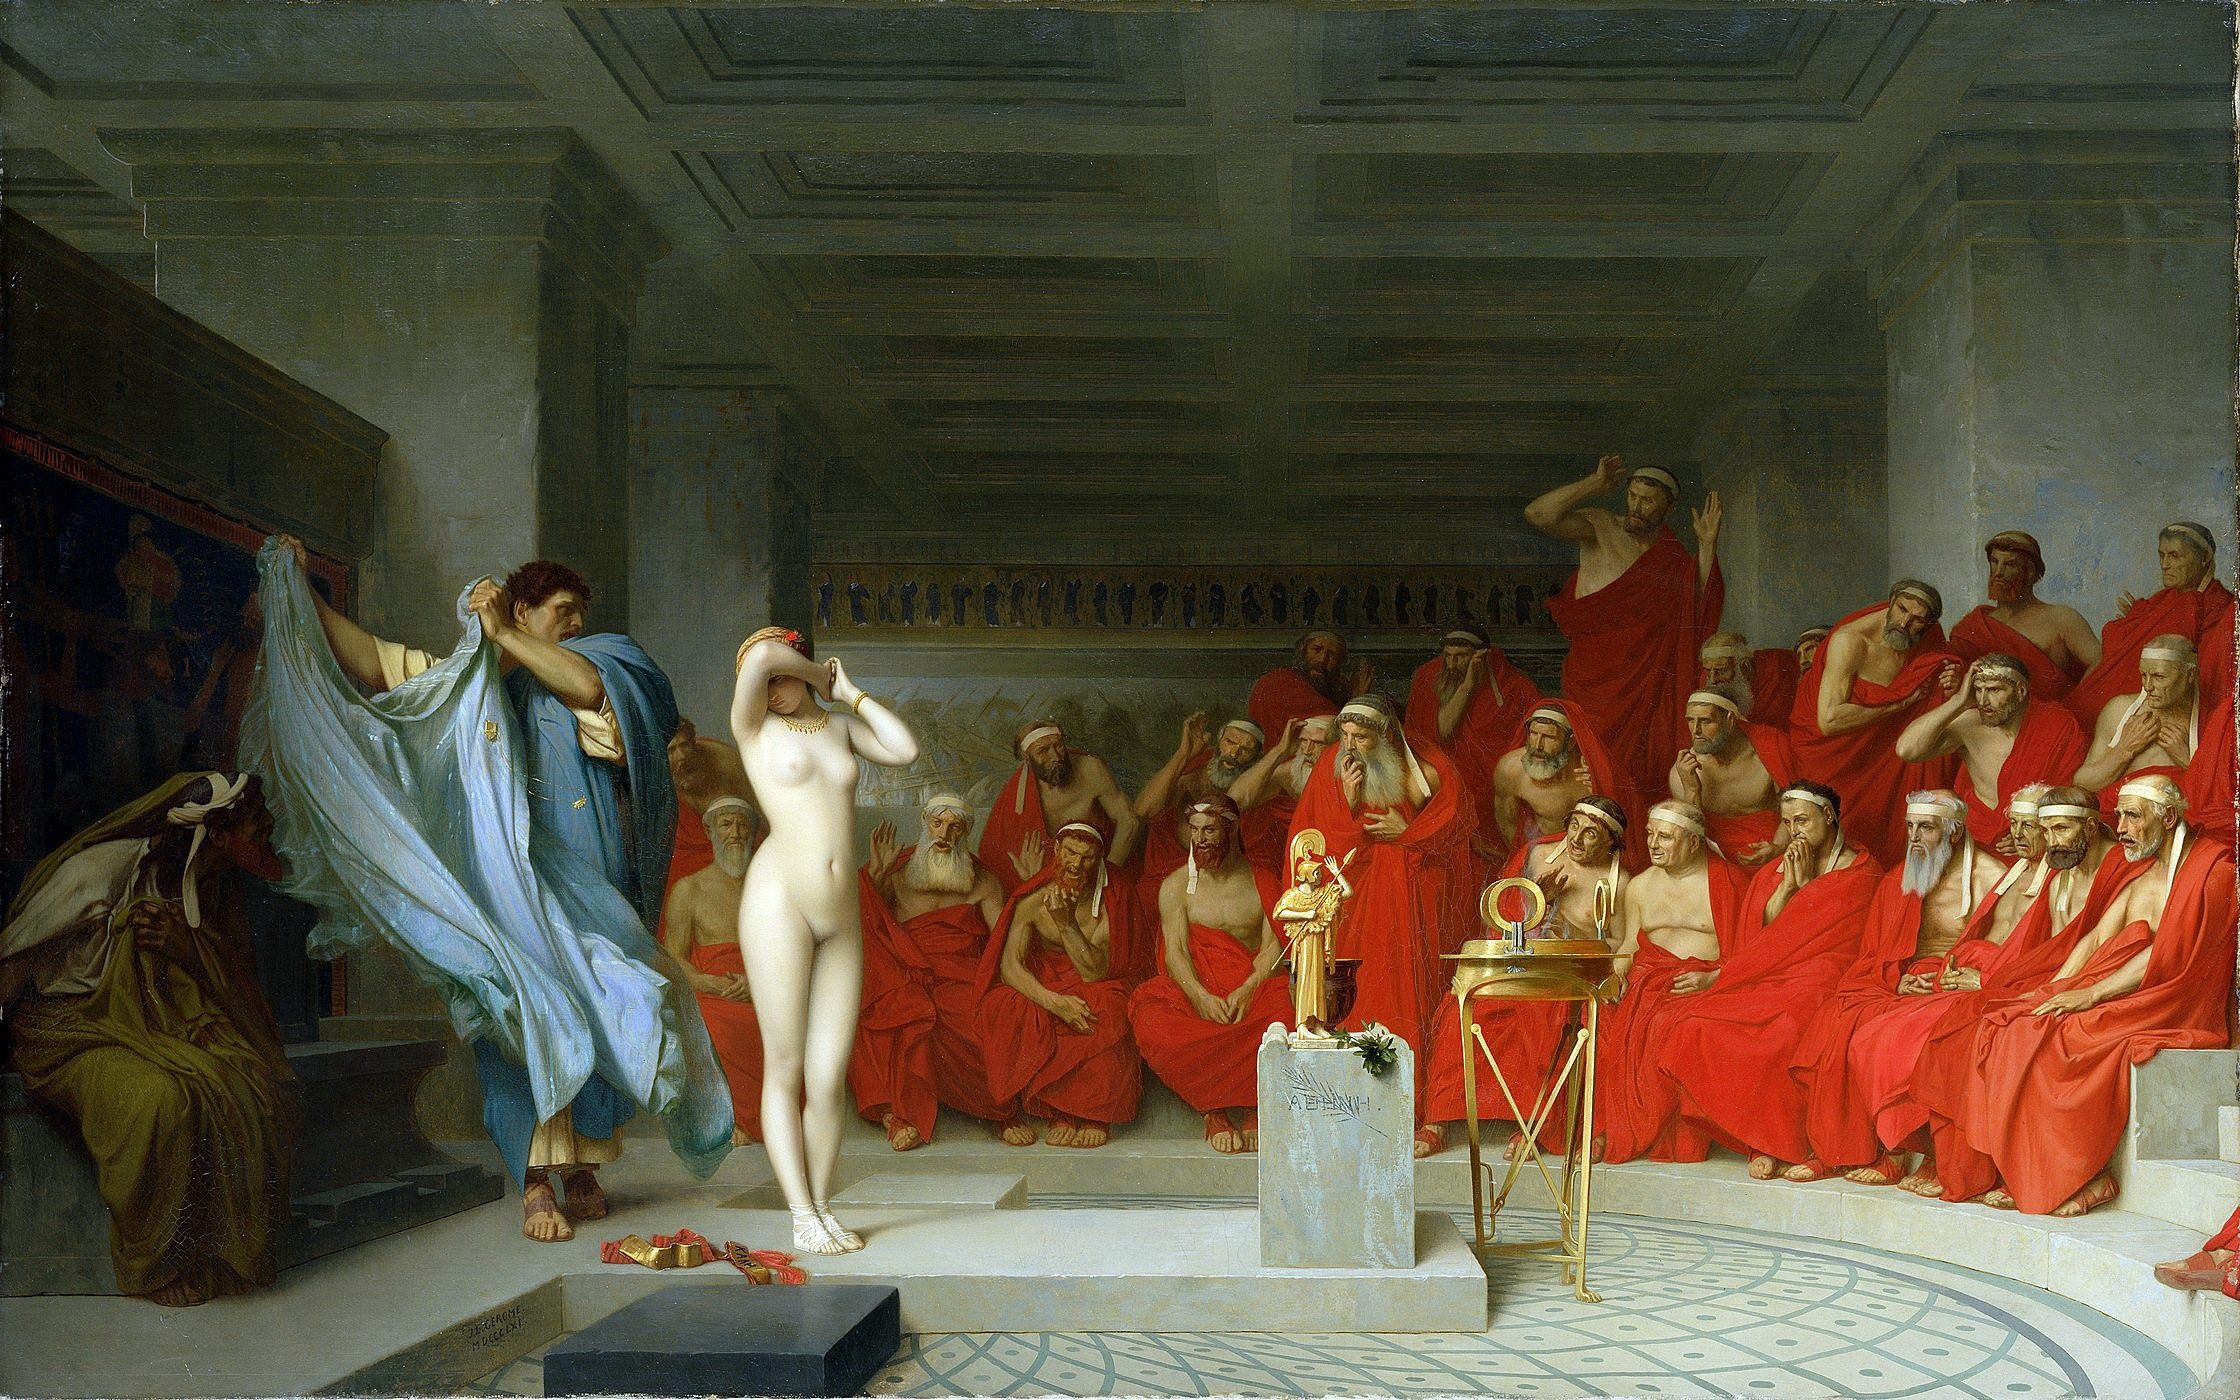
\includegraphics[height=0.3\textheight,keepaspectratio]
                          {frine.jpg}
  \caption{Friné ante o Aerópago (1861), de Jean-Léon Gérôme (\cite{gerome})}.
  \label{fig:3}
\end{figure}

\section{Rapariga lavando os pés a uma criança}

\begin{figure}
\centering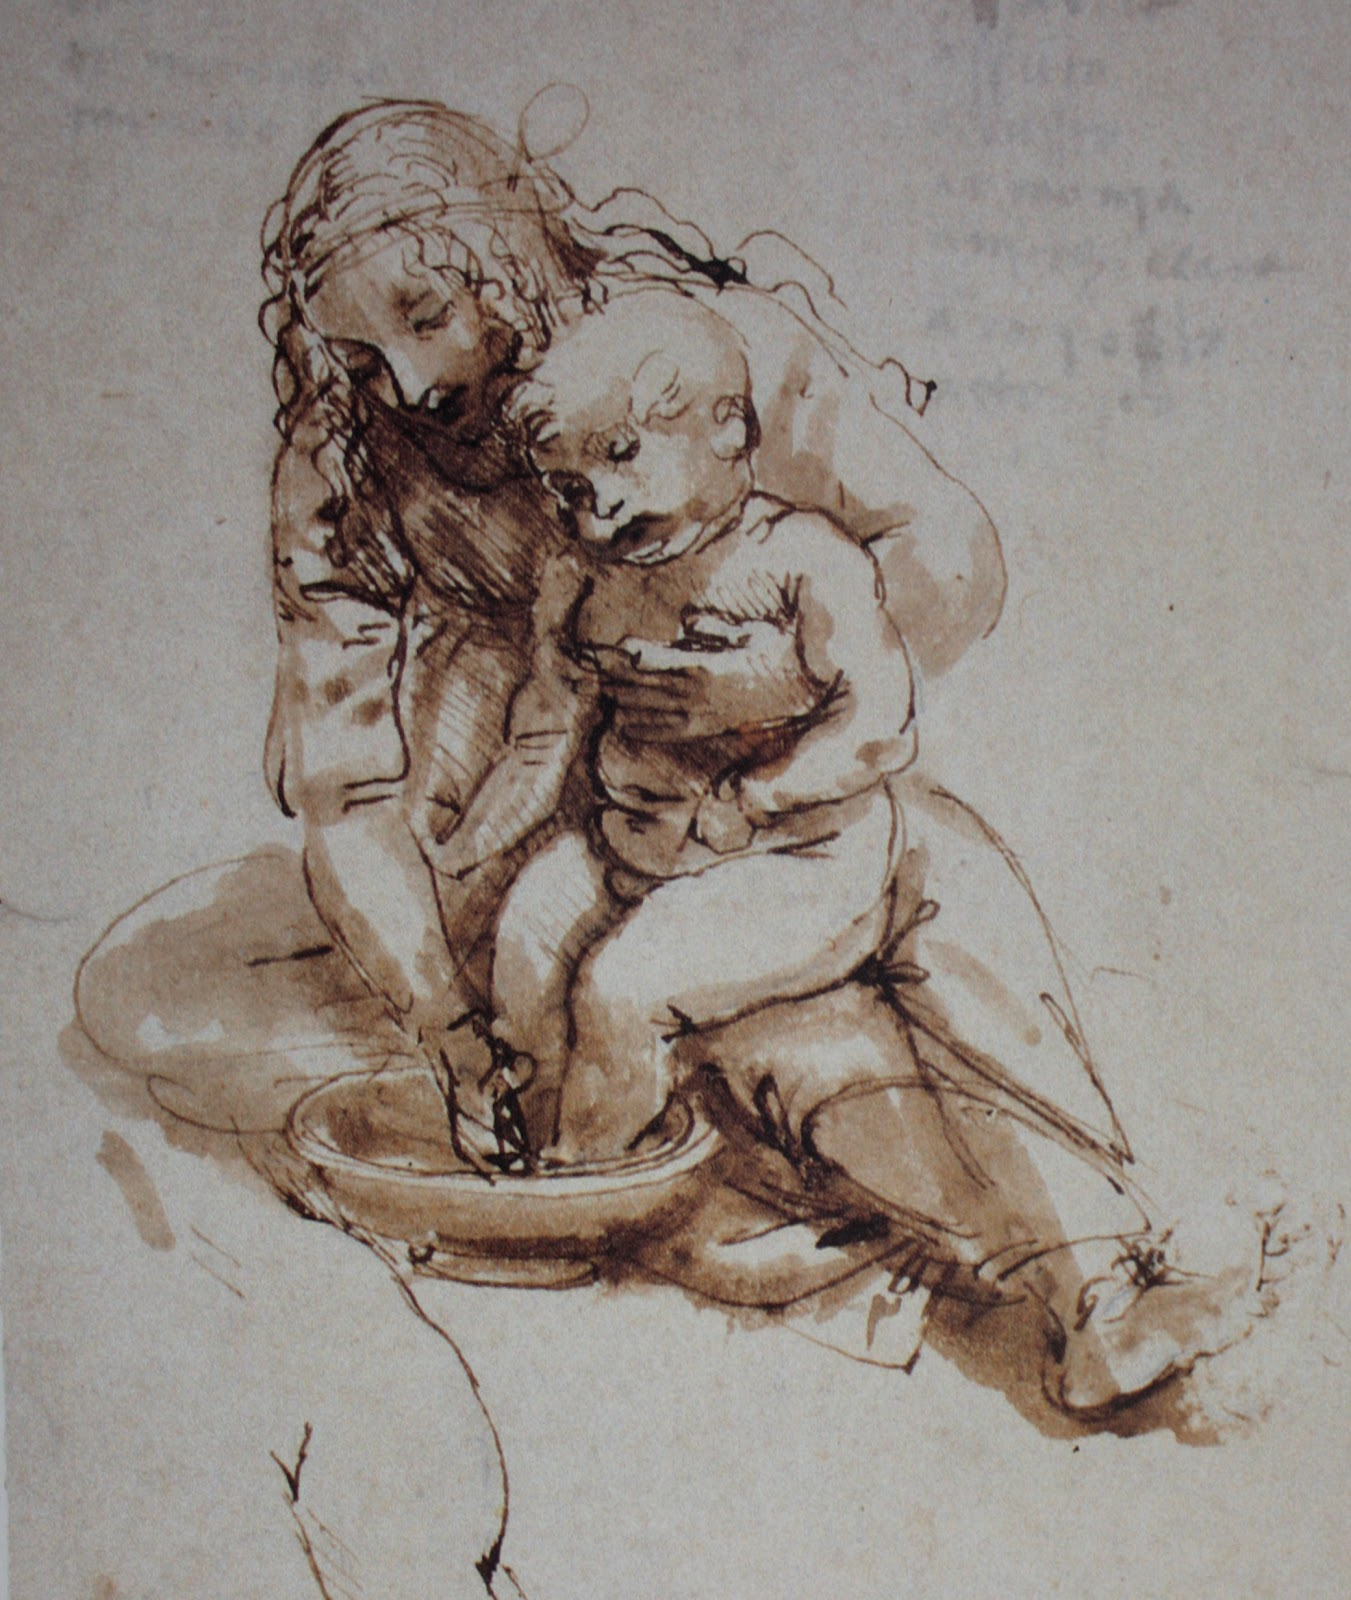
\includegraphics[height=0.3\textheight,keepaspectratio]
                          {mulher-lavando.jpg}
  \caption{Mulher Lavando os Pés a Uma Criança, Leonardo Da Vinci, ca.1480}.
  \label{fig:4}
\end{figure}

No ano 2000, o Centro Cultural de Belém, em parceria com vários museus
e instituições portuguesas, organizou uma exposição onde estiveram
patentes muitos desenhos de mestres europeus pertencentes a coleções
portuguesas. Desde então, já tive oportunidade de rever alguns deles,
mas nunca um em particular, o que é certamente o mais célebre, e que
pertence à colecção da Faculdade de Belas Artes do Porto. Felizmente
possuo dois catálogos com reproduções de boa qualidade deste desenho
(\cite{desenhos-europeus},\cite{desenhos-porto}).

Trata-se de um pequeno desenho de Leonardo da Vinci (Figura
\ref{fig:4}) que representa uma jovem mulher lavando os pés a uma
criança (a obra aparece alternadamente titulada como ``mulher
lavando'' e ``rapariga lavando'').

É a partir do século XVIII que o coleccionismo de desenhos,
particularmente desenhos dos ``grandes mestres'', começa a ganhar
fôlego no mercado da arte. Estes desenhos nunca são obradas acabadas
ou sacralizadas, e normalemente executados como estudos prévios de
pinturas, são instrumentos de trabalho, manejados, sujados de óleo,
dobrados e sobrepostos. O coleccionismo isola-os desta proveniência
instrumental e estabelece-os como obras de arte independentes, também
porque, em paralelo, elas são sujeitas a uma série de aventuras à
medida que vão trocando de dono.

A proveniência deste desenho demonstra que passou pelas mãos de
inúmeros coleccionadores, e que a sua atribuição se perdeu durante
esse período (\cite{desenhos-europeus})
\begin{enumerate}
\item Commendattore Vittorio Genevosio [Gelozzi ou Gelosi]
  (1719-1795?). Este coleccionador terá, ele prórpio, cortado e
  montado o desenho a partir da folha original de Leonardo, e aplicado
  nele a carimbo negro a marca de coleccionador.
  \item Marchese Giovanni Turinetti di Priero. A folha aparece citada
    num inventário em 1801, como sendo de Raffaellino Da Reggio.
  \item Coleccionador português não identificado
  \item Academia de Marinha e Comércio, Porto (carimbado novamente
    como marca de colecção da academia)
  \item Academia de Belas Artes, Porto
  \item Faculdade de Belas Artes do Porto
\end{enumerate}

Desconhece-se o paradeiro do desenho antes da montagem e carimbagem
iniciais. A história da dispersão da obra gráfica de Leonardo está é
bem conhecida: Francesco Melzi herdou o espólio de Leonardo, compilou
algumas obras dispersas como o \emph{Trattato della Pittura}, e o seu
filho cedeu-o a Pompeu Leoni, escultor e medalhista italiano, que,
recebendo todos os desenhos e escritos, resolveu selecioná-los e
desmembrá-los do seu contexto para os poder vender por uma soma mais
alta (\cite{wiki-leoni}).

Note-se que a atribuição foi durante muito tempo feita a um tal de
Raffaeliino Da Reggio, pintor maneirista romano do século XVI. A
confusão poderá ter advindo da proximidade entre os nomes deste pintor
e de Raffaelo da Montelupo, um escultor renascentista, que, tal como 
leonardo, era canhoto..A primeira atribuição a Leonardo foi sugerida
por Philip Pouncey em 1965, através de uma fotografia, e confirmada em
1977 pelo exame do original. Os argumentos utilizados por Pouncey
baseiam-se numa relação estilística entre o desenho do Porto e um
grupo de desenhos para uma composição da \emph{Virgem e o Menino com
  Gato} existente no Museu Britânico.

Além das marcas de sombreado executadas diagonalmente de cima para
baixo e da esquerda para a direita, que indicam obviamente um pintor
canhoto, Pouncey chama a atenção para a presença, no desenho do Porto
bem como nos desenhos do Museu Britânico, da presença vigorosa das
vfiguras, de tipos fisionómicos semelhantes e do mesmo uso rápido da
pena, bem como uma aplicação cuidadosa da aguada no sombreado. Na
mesma folha do porto encontramos também um estudo separado das nádegas
de uma criança, que se aproxima do desenho de uma criança nua na
coleção do Castelo de Windsor.

Pouncey data este desenho de 1480, pouco antes da transferência do
pintor para de Florença para Milão, embora em escritos subsequentes
Carlo Pedretti sugira que tenha sido feito depois desta. As razões
citadas por Pedretti prendem-se com a presença, no \emph{verso} do
desenho do Porto, de uma lista de palavras que coincide exactamente
com uma lista semelhante do \emph{Codex Trivulziano}, no castelo da
família Sforza em Milão, para quem Leonardo trabalhou.

\printbibliography[heading=bibliography,title={Bibliografia}]

\end{document}
